We created the topology shown in Figure~\ref{fig:topology} in ExoGENI to conduct our experiments. Among the $23$ nodes in this topology, we specify $6$ data origins and $6$ data sinks as the end hosts to transfer a batch of data files ($886$ files) of different sizes that we randomly acquired from OSG. There are $49$ links in total with which we try to emulate a topology following the power law, i.e., $4$ routing nodes in the middle to emulate the backbone domain and the rest emulate the access domains in between the backbone nodes and the end hosts. 

We ran two sets of experiments to collect two sets of training data. In the first one, called {\it Partial},
data transfers only happen between the origins and sinks. In the second one, called {\it Complete}, 
data transfers happen between all the end host pairs. Each origin node sends all the $886$ files to all the receiving nodes, where the file integrity is being checked.

For each experiment, probabilistic integrity error or network impairment via the Chaos Jungle tool is injected to the links and end hosts in sequence with the given probability setting. For each fault injection scenario, the entire set of {\it Partial} or {\it Complete} data transfers are conducted. The receiving node checks if the receiving file is identical to the original copy and marks the data transfer as failure if files are not identical. A file could also be missed which is treated as failure. We treat retransmission as a separate feature. Each link or node component with fault injected is a label and each file transfer becomes a data point in the training set. We further parallelized the data transfer process to reduce the emulation time down to about twenty four hours for this particular network. 

Following figures show the accuracy results. The figures from Decision Tree and Bayes models have two parts: the left part shows the results for the {\it Partial} data set and the right part shows the results for the {\it Complete} data set. Each part depicts four levels of accuracy: flow, top-1, top-2, and top-3. The results from the SVM show two different types of models: linear SVM and general SVM with RBF kernel.
We inject integrity errors in $67$ network components including the interfaces and end host nodes, which represents $67$ labels. As a very basic benchmark, the accuracy of random classification is merely $\frac{1}{67}$.
\begin{figure}[!ht]
\begin{center}
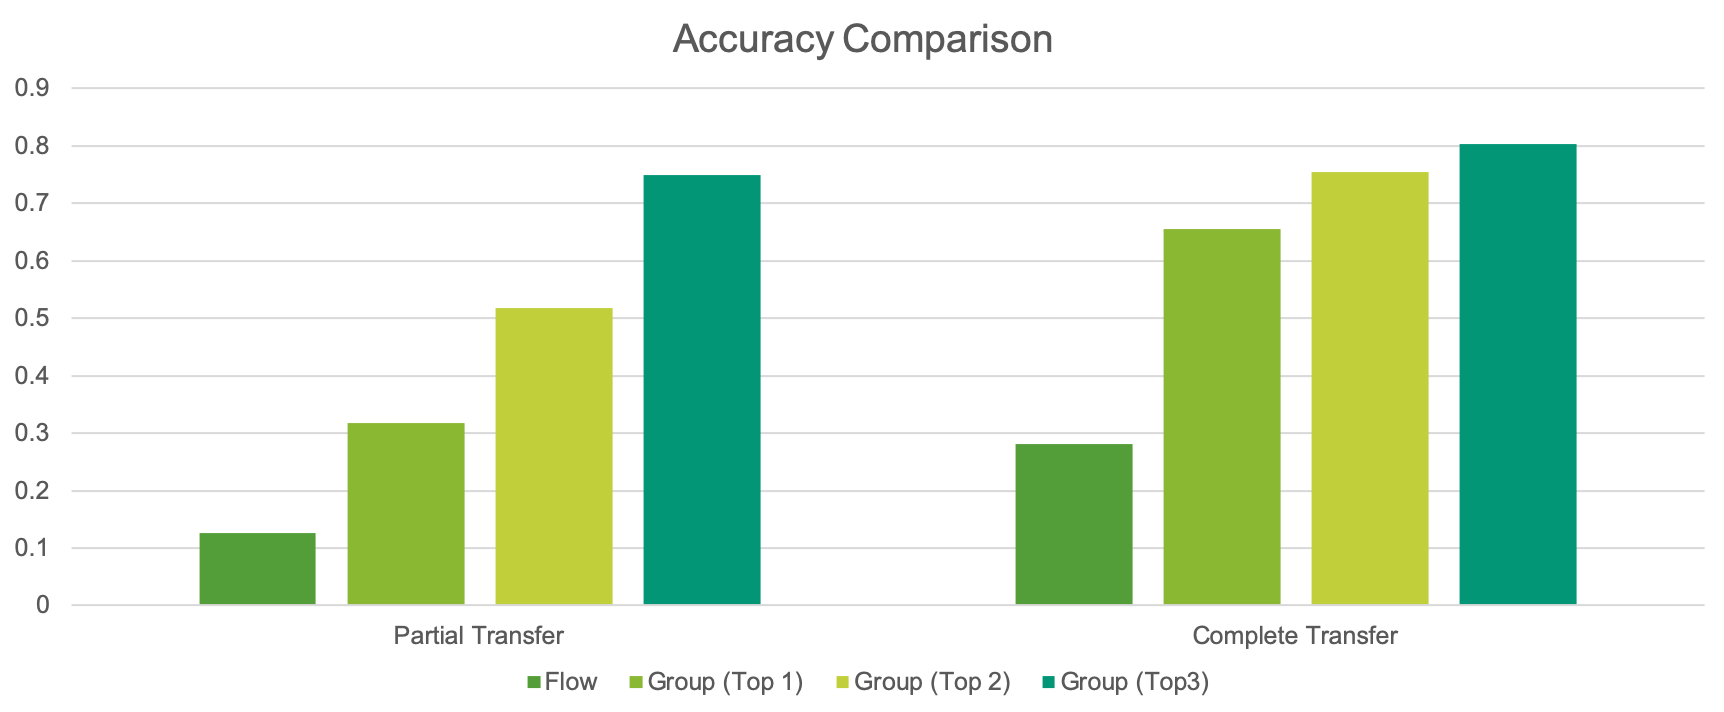
\includegraphics[width=0.45\textwidth]{./figure/dt-result}
\end{center}
\vspace{-0.05in}
\caption{Classification Accuracy with Decision Tree Model}
\vspace{-0.05in}
\label{fig:dt}
\end{figure}

Fig.~\ref{fig:dt} presents the results using the random forest model. The single flow level accuracy is very poor and the accuracy increases dramatically with bigger $k$. It also clearly shows that the model with {\it Complete} data performs much better than the {\it Partial} case. However, the gap becomes small when $k=3$. 

\begin{figure}[!ht]
\begin{center}
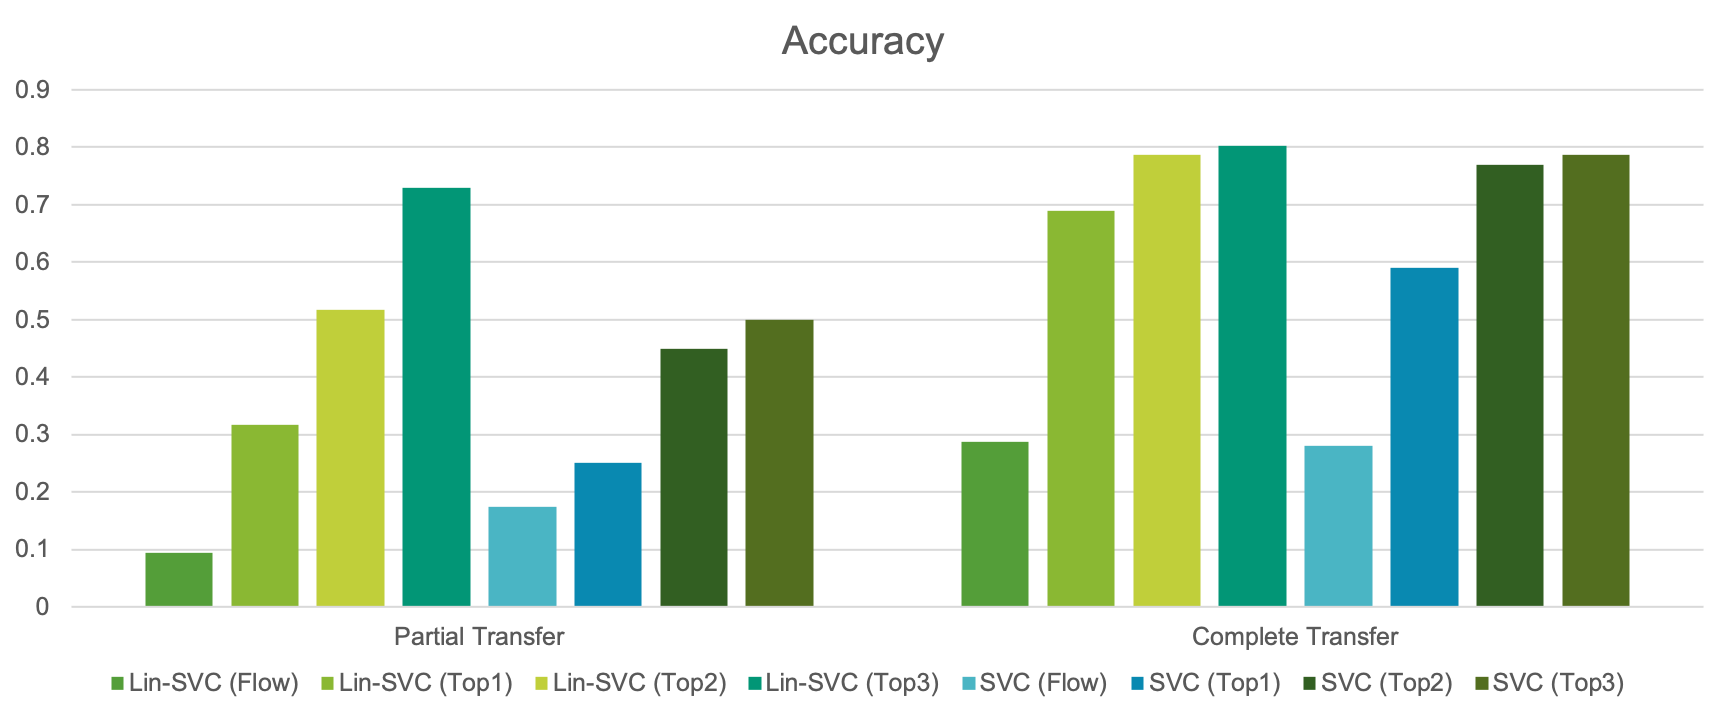
\includegraphics[width=0.45\textwidth]{./figure/svm-result}
\end{center}
\vspace{-0.05in}
\caption{Classification Accuracy with SVM Model}
\vspace{-0.05in}
\label{fig:svm}
\end{figure}

Fig.~\ref{fig:svm} depicts the results using two different models: linear and general SVM with RBF kernel. It shows the same trends with regards to $k$. It also clearly shows that Linear SVM performs better than the general SVM.
\begin{figure}[!ht]
\begin{center}
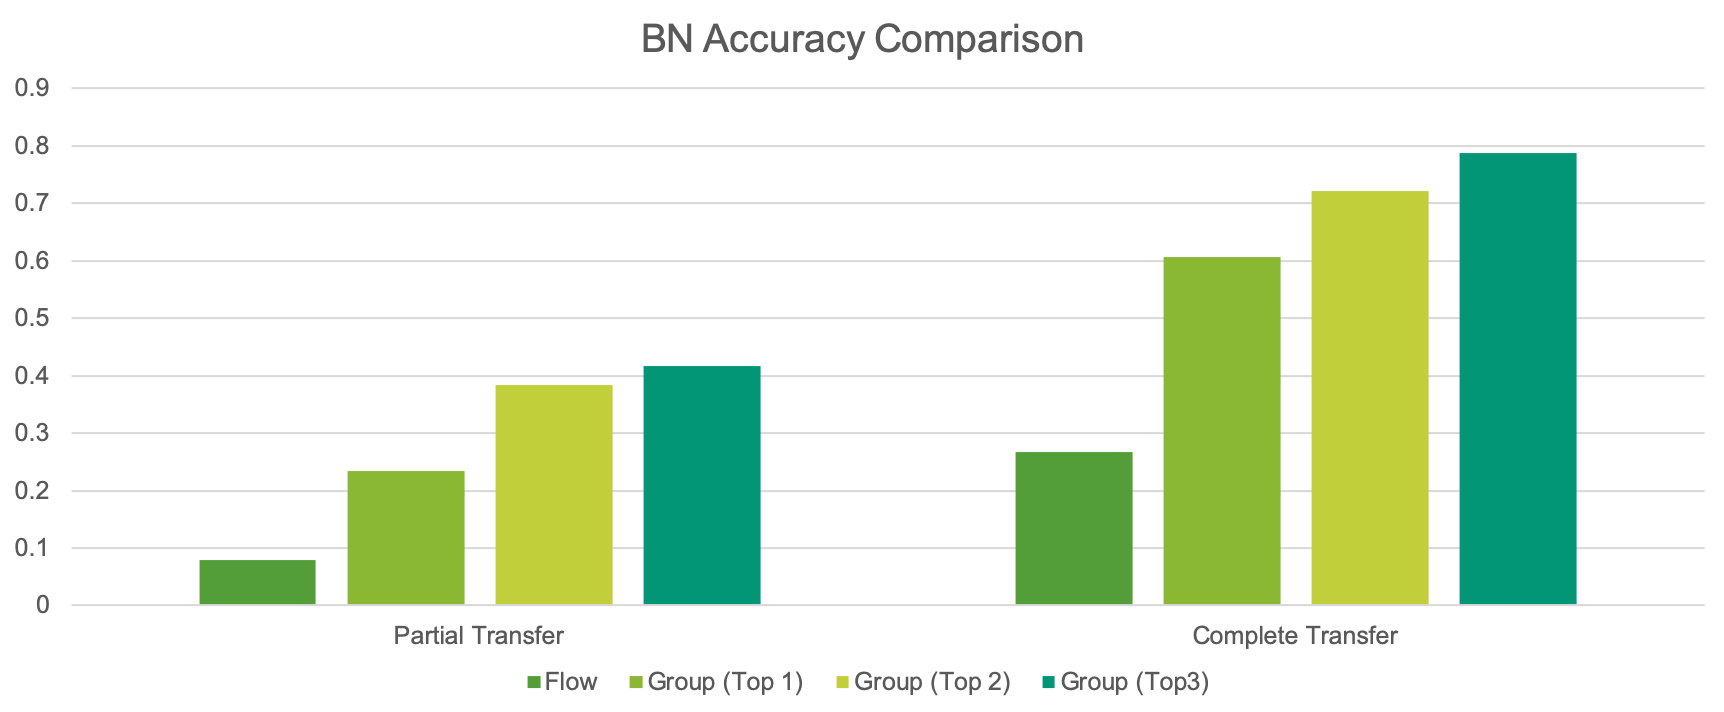
\includegraphics[width=0.45\textwidth]{./figure/bn-result}
\end{center}
\vspace{-0.05in}
\caption{Classification Accuracy with Multinomial Naive Bayes}
\vspace{-0.05in}
\label{fig:bn}
\end{figure}

Fig.~\ref{fig:bn} shows the results using the Multinomial Naive Bayes approach. Again, the accuracy increases with $k$.

When comparing between above three models, the random forest performs the best, linear SVM the next best, and the Bayes model performs the worst. 

When $k=3$, the maximal achieved accuracy is slightly above $80\%$, which is very promising for our specific network RCA problem. We tried larger values of $k$. The accuracy doesn't change much until $k$ reaches 20, when it will jump to above $90\%$. We believe the accuracy stall may be mainly due to the particular topology and more importantly the set of the end hosts for data transfers that do not include all the router nodes, which violates the necessary condition to cover all the possible failure causes in a network~\cite{netbouncer:nsdi18}.  

We next look into the training time of the above three models. From Table.~\ref{tab:time}, it is clear that SVM takes significantly longer time than the other two. Actually the SVC with the default RBF kernel takes much longer time than the linear SVC whose running time is shown in the table. Between the other two, the decision tree model takes the shortest time. Another observation is that the training with the {\it Complete} data set finishes much faster than that with {\it Partial} data set. This makes sense because more complete training data helps the model training converge faster. 

To make the evaluation complete, we also present the F-Score for the single label classification {\it Complete} case in the same table. The SVM model gets the best F-score. As we stated before, we believe the accuracy is the more meaningful metric for the RCA problem, though we will continue to explore better metrics.     
\begin{table}[!ht]
\caption{Training Time and F\-Score
\label{tab:time}}
\vspace{-0.1in}
\begin{center}
\begin{tabular}{ |c|c|c|c| } 
 \hline
  & Partial & Complete & F-Score ($k=1$)\\ 
 \hline\hline
 Decision Tree & 164ms & 95.1ms & 0.3266\\ 
 \hline
 Bayes & 416ms & 174ms & 0.3382 \\
 \hline
 SVM & 26700ms & 10300ms & 0.368 \\ 
 \hline
\end{tabular}
\end{center}
\vspace{-0.1in}
\end{table}
Combining both training accuracy and training time, the random forest model appears to be a clear winner for the studied RCA problem.